\documentclass[a4paper,10pt]{article}

\usepackage[T1]{fontenc}
\usepackage[utf8]{inputenc}
\usepackage{lmodern}
\usepackage[scale=0.92]{geometry}
\usepackage{parskip}
\usepackage{tabularx}
\usepackage{enumitem}
\usepackage{xcolor}
\usepackage{titlesec}
\usepackage{graphicx}
\usepackage[unicode,hidelinks]{hyperref}
\usepackage{fontawesome5}

\definecolor{linkcolour}{RGB}{0,80,158}
\hypersetup{colorlinks=true,urlcolor=linkcolour,linkcolor=linkcolour}
\newcolumntype{C}{>{\centering\arraybackslash}X}
\titleformat{\section}{\large\bfseries\raggedright}{}{0em}{}[\titlerule]
\titlespacing{\section}{0pt}{6pt}{4pt}
\setlength{\parindent}{0pt}
\setlist[itemize]{nosep,leftmargin=1.2em,itemsep=1.5pt,topsep=1pt,label=--}

% Bloc expérience / projet : titre à gauche, dates à droite, puis puces
\newenvironment{joblong}[2]
{\begin{tabularx}{\linewidth}{@{}X r@{}}\textbf{#1} & \textbf{#2}\\[2pt]\end{tabularx}\begin{itemize}}
{\end{itemize}}

\begin{document}
\pagestyle{empty}

% ===================== EN-TÊTE =====================
% Photo facultative : décommenter les deux lignes \includegraphics ci-dessous
% et placer photo.jpg à côté de ce fichier.
\begin{tabularx}{\linewidth}{@{}C@{}}
% 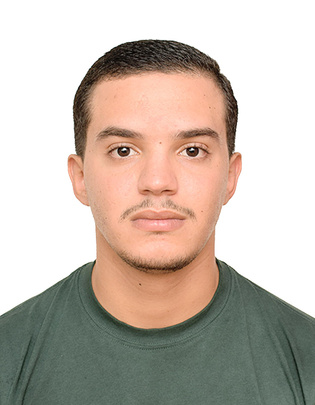
\includegraphics[height=2.6cm]{photo.jpg}\\[4pt]
{\Huge\textbf{Chems Eddine Adel KEBAILY}}\\[3pt]
\textbf{Étudiant en Master 1 Traitement du signal et des images $\mid$ Machine Learning $\mid$ Vision par ordinateur}\\[4pt]
Calais $\mid$
\href{mailto:chemseddine.keb@gmail.com}{\faEnvelope\ chemseddine.keb@gmail.com} $\mid$
\href{tel:[numéro retiré]}{\faMobile\ [numéro retiré]} $\mid$ \faCar\ Permis B\\[2pt]
\href{https://www.linkedin.com/in/chemseddineadel-keb}{\faLinkedin\ LinkedIn} $\mid$
\href{https://github.com/adkebaily}{\faGithub\ GitHub} $\mid$
\href{https://chemseddine-kebaily.netlify.app}{\faGlobe\ chemseddine-kebaily.netlify.app}
\end{tabularx}

% ===================== PROFIL =====================
\section{Profil}
Étudiant en \textbf{Master 1 Traitement du signal et des images} à l'Université du Littoral Côte d'Opale, avec une double compétence en \textbf{apprentissage automatique} et en \textbf{développement logiciel}. Réalisation de projets de classification (détection de phishing avec scikit-learn, reconnaissance de 90 espèces animales par \textbf{Vision Transformer} et transfer learning sous PyTorch) et de deux stages chez \textbf{Ooredoo Algérie} en développement web (Spring Boot, React, SQL/Oracle) et mobile (Flutter), en méthode Agile. Intérêt marqué pour le traitement d'images, la vision par ordinateur et les agents IA.

% ===================== FORMATION =====================
\section{Formation}
\begin{tabularx}{\linewidth}{@{}p{0.18\linewidth} X@{}}
2026 -- 2027 & \textbf{Master 1 Traitement du signal et des images} (en cours), Université du Littoral Côte d'Opale (ULCO) \\
2022 -- 2025 & \textbf{Licence Systèmes informatiques}, Université M'Hamed Bougara de Boumerdès \\
2022 & \textbf{Baccalauréat Techniques mathématiques, Génie civil} (mention Bien), Lycée Ali Chekiri, Chéraga \\
\end{tabularx}

% ===================== EXPÉRIENCES =====================
\section{Expériences professionnelles}

\begin{joblong}{Stagiaire développement mobile — Ooredoo Algérie}{Déc. 2024 -- Janv. 2025}
\item Participation au développement d'applications mobiles multiplateformes avec \textbf{Flutter}.
\item Contribution à l'ensemble des étapes du cycle de développement en méthode \textbf{Agile} : analyse du besoin, développement, tests et revue.
\item Découverte de l'infrastructure datacenter et des architectures \textbf{cloud hybrides} (GCP et on-premise).
\end{joblong}

\begin{joblong}{Stagiaire développement web — Ooredoo Algérie}{Déc. 2023 -- Janv. 2024}
\item Développement de l'application web de gestion des flux de trésorerie des terminaux de paiement (POS) avec \textbf{Spring Boot} et \textbf{React}.
\item Analyse et exploitation des données par requêtes \textbf{SQL} ; maintenance et optimisation de bases \textbf{Oracle}.
\item Intégration d'évolutions fonctionnelles, \textbf{tests unitaires}, documentation technique, revues de code et versioning Git.
\end{joblong}

% ===================== PROJETS =====================
\section{Projets académiques}

% TODO : remplacer les deux liens ci-dessous par les vraies URL (rapport Drive, dépôt GitHub)
\begin{joblong}{Détection de phishing par apprentissage automatique — PFE de Licence (recherche)}{2025}
% À VÉRIFIER : détails ajoutés, à adapter à ce que tu as réellement fait
\item Constitution d'un jeu de données, extraction de caractéristiques et comparaison de plusieurs modèles de classification avec \textbf{Python} et \textbf{scikit-learn}.
\item Évaluation des modèles (précision, rappel, F1-score) et rédaction d'un rapport de recherche. \href{https://drive.google.com}{\faFilePdf\ Rapport}
\end{joblong}

\begin{joblong}{Reconnaissance d'animaux (90 espèces) — Vision par ordinateur}{}
% À VÉRIFIER : ajouter l'année et ajuster les détails
\item Classification d'images multi-classe par \textbf{Vision Transformer (ViT)} pré-entraîné et \textbf{transfer learning} sous \textbf{PyTorch}.
\item Préparation et augmentation des données, entraînement sur GPU (Google Colab, Kaggle) et analyse des résultats. \href{https://github.com/adkebaily}{\faGithub\ Code}
\end{joblong}

% ===================== COMPÉTENCES =====================
\section{Compétences}
\begin{tabularx}{\linewidth}{@{}>{\bfseries}p{0.25\linewidth} X@{}}
IA \& data & PyTorch, TensorFlow, scikit-learn, Vision Transformer, transfer learning, classification, Kaggle, Google Colab \\
Langages & Python, C, C++, Java, JavaScript, PHP, SQL (Oracle), HTML/CSS \\
Développement & Spring Boot, React, Node.js, Flutter, API REST \\
Systèmes \& réseau & Linux (Ubuntu), Windows Server, VirtualBox, Cisco Packet Tracer \\
Outils \& méthodes & Git/GitHub, VS Code, IntelliJ IDEA, WampServer, Photoshop ; Agile, revues de code, tests unitaires \\
Savoir-être & Organisation, communication, autonomie, adaptabilité, esprit d'équipe \\
\end{tabularx}

% ===================== ACTIVITÉS =====================
\section{Activités associatives et formations}
\begin{tabularx}{\linewidth}{@{}p{0.18\linewidth} X@{}}
2025 -- 2026 & \textbf{Co-manager du département Visual} — DevUp Club, Université de Boumerdès \\
2024 -- 2025 & \textbf{Membre du département Développement} — DevUp Club, Université de Boumerdès \\
Févr. 2025 & \textbf{Bootcamp « AI to Fullstack »} — DevUp Club, Université de Boumerdès (mention Très bien) \\
\end{tabularx}

% ===================== LANGUES =====================
\section{Langues}
\textbf{Arabe :} natif \hfill \textbf{Français :} B2 \hfill \textbf{Anglais :} B2

\end{document}
